
\hypertarget{working_editor}{}
\section{Keystrokes (Editor)}
\index{editor}
\index{editor!keystrokes}

\begin{figure}[H]
  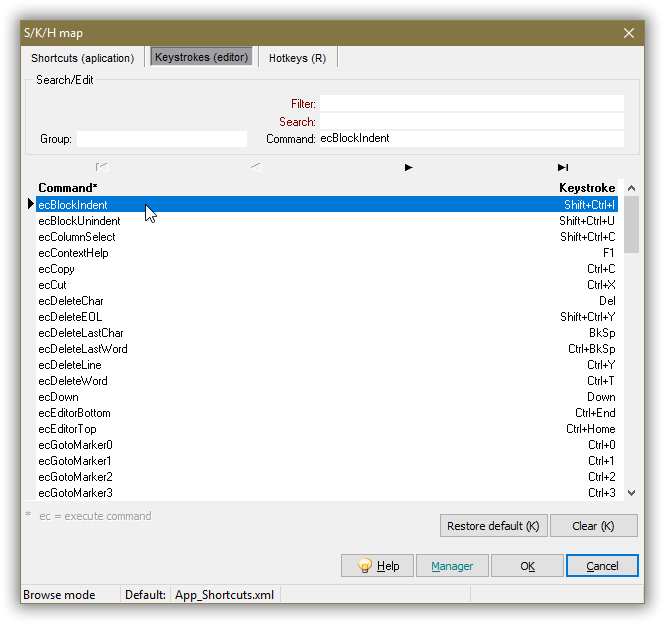
\includegraphics[scale=0.35]{./res/skh_map_keystrokes_dlg.png}\\
  \caption{Keystrokes (Databases).}
  \label{fig:keystrokes_dlg}
\end{figure}

This interface
(Figure \ref{fig:keystrokes_dlg})
allows to change the default SynEdit keystrokes.
It is possible only change the keystroke associaed to any \texttt{ecAction} (execute command action).
A set of user friendly keystrokes gives high productivity leading with
all instances of the class \textit{SynEdit}: Editor, IO and LOG.

Read below for a brief description of available buttons (Figure \ref{fig:keystrokes_dlg}):

\begin{quote}
  \begin{footnotesize}
    \begin{description}
      \item[Restore default (K):]
        Restores the file \texttt{Editor\_Keystrokes.xml} from the origin at
        (\texttt{InstallPath/data/data.zip}). Any prior change to the file ini file
        \texttt{Editor\_Keystrokes.xml} being used will be lost.
      \item[Clear (K):]
        Clear the selected keystroke.
    \end{description}
  \end{footnotesize}
\end{quote}
